\documentclass[a4paper,12pt,notitlepage]{report}
\usepackage[T1]{fontenc}    % Codifica dei font latini
\usepackage[utf8]{inputenc} % Lettere accentate da tastiera
\usepackage[english]{babel} % Lingua del documento  
\usepackage{graphicx}
\usepackage{caption}

\graphicspath{{images/}}    % Specifica la cartella con le immagini

\author{Matteo Colombo \and Andrea Troianiello}
\title{NonSoloLibri}



\usepackage{hyperref}       % Per collegamenti ipertestuali, 
\hypersetup{hidelinks}      % Rimuove riquadri dai collegamenti                     

\begin{document}


\begin{titlepage}           % Compone la pagina iniziale
    \centering
    {\Large Internet of Things}\\[4em]
    
\includegraphics[width=7cm]{polimi.png}\\[8em]
    {\Huge Waste Management System}\\[4em]
    {\large MATTEO COLOMBO - 883114 - 10459278}\\[1em]
    {\large ANDREA TROIANIELLO - 898113 - 10455250}\\[4em]
    \today
\end{titlepage}


% ------------------------- % Inizio del contenuto
% ------------------------- % Fine del contenuto
\section*{Introduction}
While developing the project we made the following assumptions:
\begin{enumerate}
    \item Coordinates are expressed in meters and they are in the range [0,1999].
    \item When the truck is traveling to a bin, it ignores all the alert messages.
    \item Alert messages are repeated every 10 seconds even by the bin where the truck is moving to.
    \item When a bin receives a Move request, it sets a lock, so that other Move requests from other nodes are rejected.
    \item If a bin in Normal status accepts a Move request and then, with the trash redirected from another mote,
        becomes full, it will still accept the trash and send itself a new Move request.
\end{enumerate}

\section*{Communication Channels}
To distinguish between bin-bin and bin-truck communication, we decided to use two channels, the first one (Channel 6) dedicated
to bin-bin messages and the second one (Channel 7), dedicated to truck-bin messages.

\section*{Components}
We decided to create two components:
\begin{description}
    \item[WMSMote:] It is the main component that depending on its ID can be either a truck or a bin.
    \item[BinSensor:] It is a non-bootable component that represents the sensor placed on each bin that signals an event every time some trash is added. 
\end{description}

\section*{BinSensor}
A BinSensor simulates the sensor which measures the quantity of trash that is added in the bin at every iteration.

Every time some trash is generated, an event containing the number of new units is emitted.

To work it uses a timer, which every time is set with a different (random) value in the range [1,30]s.\\[1em]
\begin{center}
    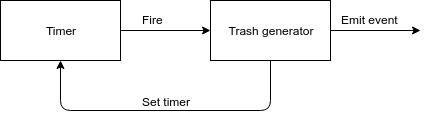
\includegraphics[scale=0.7]{sensor.png}
\end{center}

\section*{WMSMote}
The WMSMote is the main component of the project and includes the logic and implementation of both the truck and the bins.

This is due to the fact that TOSSIM is not capable of handling heterogeneous networks. Therefore a node whose ID is 0 will be a truck,
while a mote with an ID greater than 0 will be a bin.
\\\\
They both share some code and respond to some common events, but have different behaviours.

\paragraph{The Truck}
has a simple behaviour which can be represented by this finite state machine:

\begin{center}
    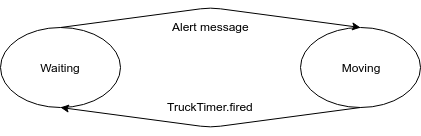
\includegraphics[scale=0.7]{truck.png}
\end{center}

When the truck is waiting, it listen for Alert messages and when the first arrives it starts traveling and sets the variable \emph{moving=true}. 
If other alerts arrive while the truck is moving, they are ignored.

The \emph{TruckTimer.fired} event is used to simulate the travel, when it fires it means that the truck is arrived to destination.

At destination the truck can empty the trash and notify the bin. Then it acquires the coordinates, releases the lock on \emph{moving} and starts again to listen.

The truck listens only to messages on the truck-bin channel, while even if he receives those on the bin-bin channel, it ignores them.

\paragraph*{The Bin} has a more complex behaviour compared to the truck, as it communicates on two channels and has more states.

\begin{center}
    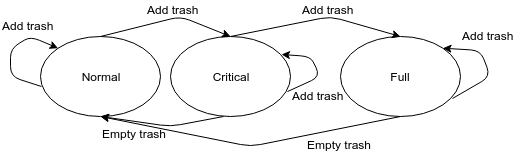
\includegraphics[scale=0.7]{bin.png}
\end{center}

The event \emph{Add trash} is emitted by the BinSensor and depending on the current state, it is handled in different ways.

If there is a state change when the trash level is increased, the mote may start alerting the truck os redirecting trash to neighbours.
\\\\
A Bin Mote is always listening on two channels, on the truck channel is listening for arrival notifications of the truck so that it can be emptied,
while on the bin-bin channel it is waiting for Move requests from other bins.

When the trash outside a bin is greater than zero, the bin sends a broadcast Move message to its neighbours and starts a \emph{MoveTrashTimer}. When this fires, it checks if at least a
neighbour bin responded and if so it sends trash to the closer one.

When a bin receives a Move request, it checks its internal status and if its Normal it starts a \emph{MoveResTimer} whose timeout depends on the distance. When it fires it responds to the mote which made the move request.

When a mote accepts to receive trash from another bin, it sets a lock so that if it receives other Move requests from other nodes they are ignored. To avoid deadlocks, there is a timer after which the lock is released and the node starts to listen again for Move requests.

\section*{Implementation and Testing}
The application was completely implemented with TinyOS, TOSSIM and TOSSIM-Live, moreover its code is completely documented.

For the simulation part we did two tests, the first one with the topology and noise trace provided at lesson, and the second one with a completely new topology and noise trace.

\end{document}